%!TEX root = ../../Master.tex
\subsection{Pratical Implementation of Graph Theory when Mapping a Building}

\subsubsection{Representing a Floor}

Every decision and every change direct is a vertex in our graph, is modelled by vertices connected with edges. \label{e_vertex} Any vertex that connects a floor with another, is called an exit vertex, and can be classified as stairs, elevators or 'others', which could be ground floor entrances or second floor walkways. Vertices that does not classify as one of the previously mentioned are doors, intersection and other positions where a change of direction can occur. Connecting the vertices are edges with a weight, which could be weighted with the distance in meters from one vertex to another. Figure \ref{fig:floorplan_graf} illustrates how the graph will look like on a floor plan for a existing building. The circles are vertices and lines are edges.

\begin{figure}[ht!]
    \centering
    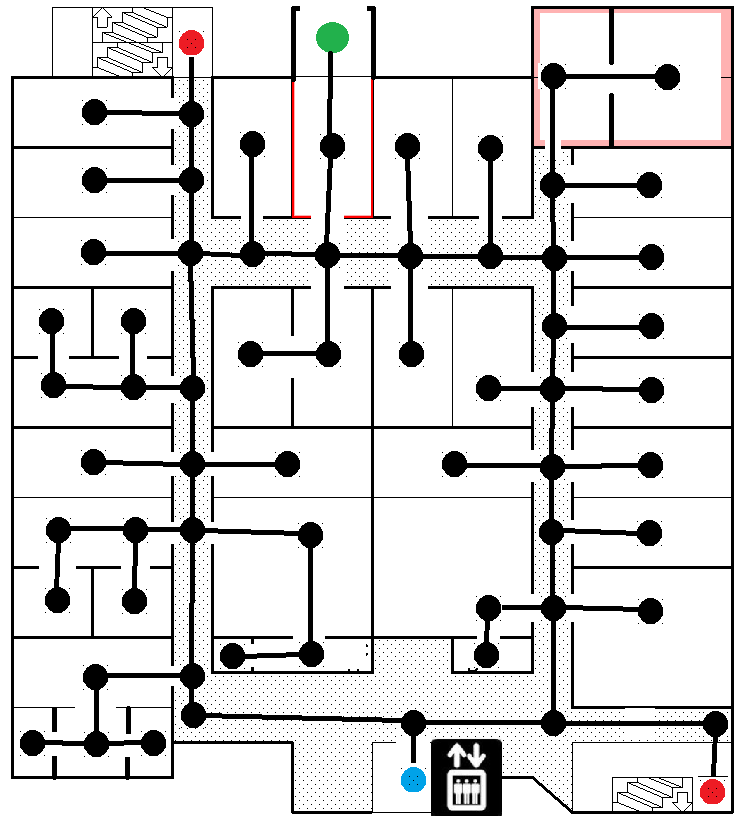
\includegraphics[width=0.5\textwidth]{floorplan_graf}
    \caption{representation of a graph on a floor plan.}
    \label{fig:floorplan_graf}
  \end{figure}
\
\subsection{Multiple Layer Handling} \label{multlayhan}

When using A* to find a path, the use of a euclidean heuristic becomes problematic when traversing multiple floors in a building. Figure \ref{fig:buildingAstar} helps illustrate this. If a euclidean heuristic is used, the algorithm will, whenever it enters a new floor, move towards the vertex (b) that is directly below the desired goal (a), regardless of whether it is an exit vertex or not. See \cref{e_vertex}. After this point has been reached, the A* algorithm will expand the search from this vertex. This will immensely decrease the usefulness of the euclidean heuristic, to a point where the A* might no longer preferable to Dijkstras algorithm. Because a low runtime is required for the solution, a better way of traversing floors must be employed.

\begin{figure}[ht!]
    \centering
    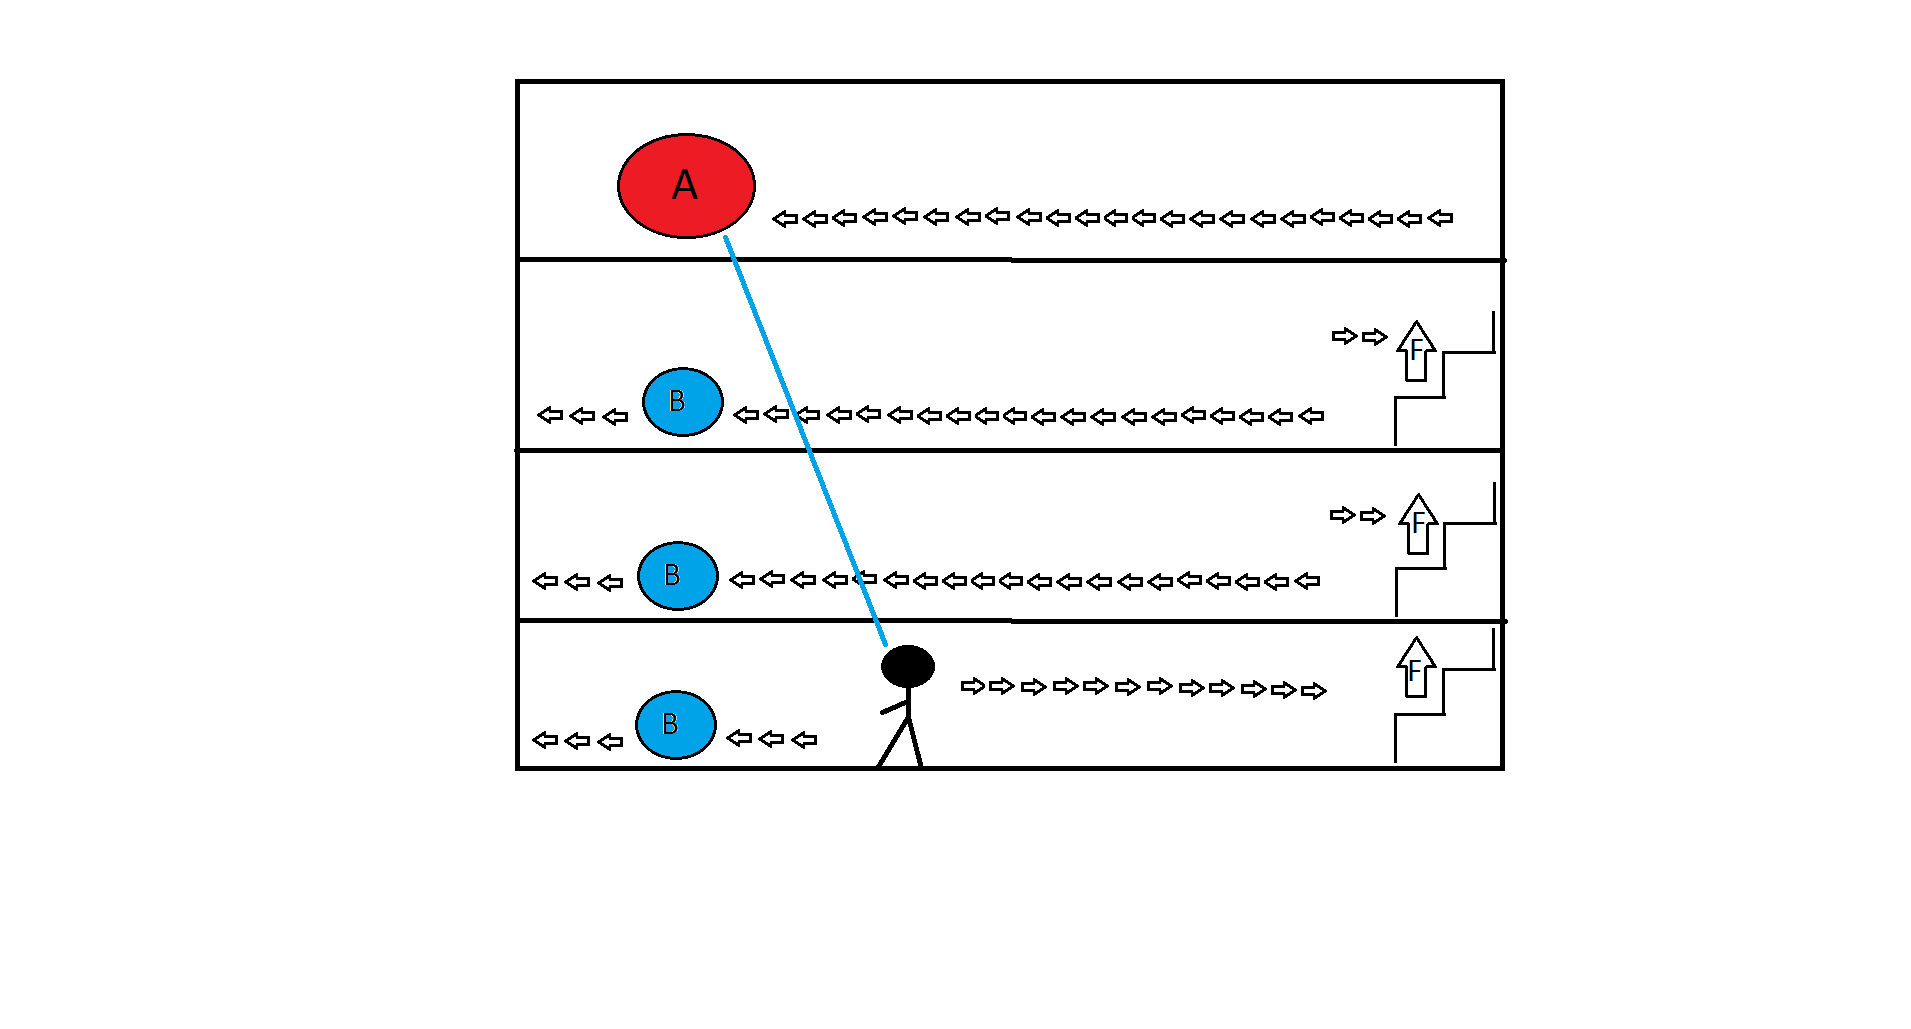
\includegraphics[width=0.5\textwidth]{buildingastar_paint}
    \caption{How many vertices the A* algorithm would expand, if using the euclidean distance as heuristic}
    \label{fig:buildingAstar}
  \end{figure}

The solution to this problem lies in a tripartitioning of the pathfinding process, and is illustrated in figure \ref{precomp}. Using the fact that the optimal route from one exit vertex to any other exit vertex is static, and only the choice of exit vertices varies when finding the omptimal route between the intial and final floor, the paths from exit vertex to exit vertex can be precomputed. By computing and storing these routes when initializing the program, the response time when prompted for a path, will be lowered significantly.

When using this approch, the runtime will consist of a round of A* runs done on both the intial floor and the destination floor. These runs are done from the start vertex and the destination vertex to all exit vertices on their respective floors. When this has been computed, all the possible combinations of paths will have their individual evaluation values added, and a comparison between the total evaluation values will dertermine the optimal path across the multiple floors.

\begin{figure}[ht!]
    \centering
    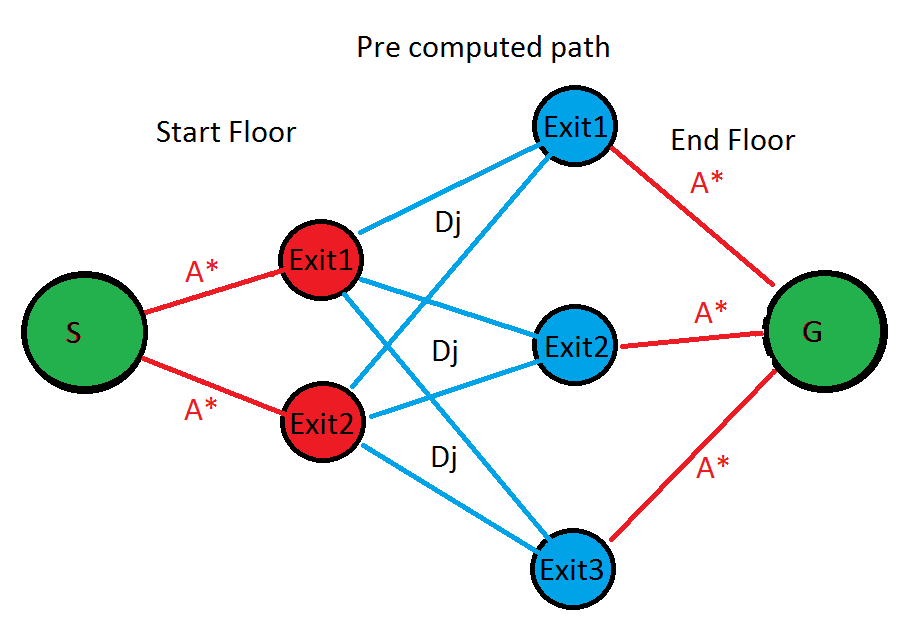
\includegraphics[width=0.5\textwidth]{precomputedpath}
    \caption{mangler billedtekst}
    \label{fig:precomp}
  \end{figure}

\kanote{mangler billedtekst}

\subsubsection{Multiple Buildings}

The previously described method for modeling floors allows the algorithm to comprehend complexes of multiple buildings, as seen in \cref{fig:PekhoeS}. The numbers indicate the different floor id's and the letters indicates the connections between the floors. Connection d shows a curved line between 5 and 4 which means they are connected.\newline

If a building with three floors and one with two floors are to be represented, the floors will be numbered 1 through 5. The building with the three floors could have its first floor numbered 1, second numbered 2 and third numbered 3. The building with two floors would then have its first floor numbered 4 and second floor numbered 5. When modelled, the floors will be sorted by their vertex id's and stacked as seen on the figure. This means that the second floor in two separate buildings will not have the same floor id. This simplifies a lookup if an individual is on the destination floor height physically, but not in the right building, because the actual floor height is not relevant as they have been numbered.\kanote{Beskriv fodelene ved at undgå dette - det er ikke for at gøre det simpelt} The thick straight line between 3 and 4, indicates a separation between two buildings, but is only present in this illustration and only indirectly included in the implementation. As seen on the figure, there is an exit vertex(a) at floor 1 connected to an exit vertex at floor 2, which could represent a stairway or an elevator. The connection(c) between 1 and 4 is possible as both of these floors is at ground level. There is also a connection(b) between 2 and 5 even though the floors are not at ground level or in the same building. This could be a representation of a walkway connecting them.
\annote{fig 4.4 boer vaere under Multiple buildings og ikke under Pathfinding Algorithms}
\begin{figure}[ht!]
    \centering
    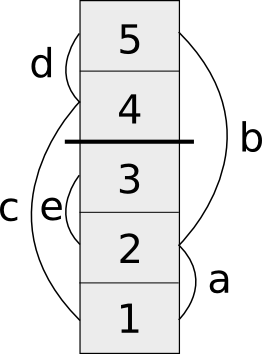
\includegraphics[width=0.5\textwidth]{PekhoeS}
    \caption{Visual representation of floors}
    \label{fig:PekhoeS}
  \end{figure}
